\documentclass[11pt]{article}

\usepackage[utf8]{inputenc}

\usepackage[a4paper,margin=1in]{geometry}

\usepackage{graphicx}

\usepackage{booktabs}

\usepackage{longtable}

\usepackage{array}

\usepackage{float}

\usepackage{caption}

\usepackage{pdflscape}

\usepackage{hyperref}

\hypersetup{colorlinks=true,linkcolor=blue,urlcolor=blue,citecolor=blue}

\begin{document}

\section*{C\&G Figures and Tables Replacement Package}

This file contains the full table contents and all figure captions generated from the current standalone experiment bundle. All numerical values are embedded directly in the LaTeX source rather than referenced externally through CSV files.

\section*{Tables}

\begin{longtable}{p{3.2cm}p{3.3cm}p{7.2cm}}
\caption{Dataset, task, and split configuration used in the current C\&G experiment line.}\label{tab:t1}\\
\toprule
Item & Value & Rationale / usage \\
\midrule
\endfirsthead
\toprule
Item & Value & Rationale / usage \\
\midrule
\endhead
Dataset file & EGMS\_L3\_E32N34\_100km\_U\_2018\_2022\_1.csv & EGMS sparse point archive used throughout the standalone project \\
Number of EGMS points & 128757 & Raw sparse samples before gridding \\
History columns & 300 columns from index 11 & Canonical input history used by all aligned experiments \\
Target column & Column 312 & Single target map forecasted after the 300-step history window \\
Grid size & 256 x 256 & Canonical dense-task grid for the main benchmark \\
Canonical interpolation & linear & Default interpolation used by the main benchmark \\
Main split protocol & spatial\_tile, tile size 32 & Leakage-aware evaluation protocol \\
Nominal split ratios & 70\% / 15\% / 15\% & Train / validation / test \\
Eligible grid cells & 53427 & Valid target cells with sufficient history coverage \\
Seed-42 train / val / test cells & 37443 / 7856 / 8128 & Representative canonical split; counts vary slightly across seeds \\
Train patch count across seeds & 643 to 659 & Variation induced by leakage-aware spatial-tile sampling across the five canonical seeds \\
Validation patch count across seeds & 169 to 187 & Patch counts used for early stopping under the same five-seed protocol \\
Repeated seeds & 42, 43, 44, 45, 46 & Mandatory multi-seed set for C\&G summaries \\
\bottomrule
\end{longtable}

\begin{longtable}{p{3.3cm}p{2.4cm}p{1.1cm}p{1.3cm}p{1.3cm}p{1.6cm}p{1.6cm}p{3.0cm}}
\caption{Main benchmark under the canonical 256 x 256 spatial-tile protocol. Negative values in the relative-change column indicate improvement over LASSO.}\label{tab:t2}\\
\toprule
Model & Family & Seeds & RMSE mean & RMSE std & Delta vs LASSO & Runtime (s) & Status / role \\
\midrule
\endfirsthead
\toprule
Model & Family & Seeds & RMSE mean & RMSE std & Delta vs LASSO & Runtime (s) & Status / role \\
\midrule
\endhead
Hybrid CNN-LSTM (1-layer) & Hybrid recurrent & 5 & 1.3077 & 0.0927 & -5.48\% & 529.86 & Proposed main model \\
Hybrid CNN-TCN & Hybrid temporal CNN & 5 & 1.3782 & 0.0685 & -0.39\% & 61.61 & Strong deep comparator \\
Temporal linear hybrid v2 & Hybrid linear-spatial & 5 & 1.3602 & 0.0917 & -1.69\% & 14.37 & Round-2 hybrid benchmark \\
LASSO & Sparse linear baseline & 5 & 1.3836 & 0.0603 & 0.00\% & 6.97 & Strongest classical baseline \\
Persistence & Naive temporal baseline & 5 & 1.5589 & 0.0954 & 12.67\% & 0.00 & Reference baseline \\
Random forest & Tree ensemble & 5 & 1.5229 & 0.1421 & 10.07\% & 110.70 & Nonlinear baseline \\
LightGBM & Boosted tree ensemble & 5 & 2.0629 & 0.4739 & 49.10\% & 5.85 & Tree + SHAP baseline \\
Linear trend & Temporal trend baseline & 5 & 2.0025 & 0.0733 & 44.73\% & 0.06 & Simple extrapolation baseline \\
\bottomrule
\end{longtable}

\begin{landscape}

\begin{longtable}{p{2.5cm}p{2.8cm}p{2.5cm}p{2.4cm}p{0.9cm}p{1.2cm}p{1.2cm}p{3.8cm}}
\caption{Deep-model repair and architecture search history. The table explicitly separates obsolete broken runs from repaired and later hybrid formulations.}\label{tab:t3}\\
\toprule
Phase & Model & Sample formulation & Target formulation & Seeds & RMSE mean & RMSE std & Interpretation \\
\midrule
\endfirsthead
\toprule
Phase & Model & Sample formulation & Target formulation & Seeds & RMSE mean & RMSE std & Interpretation \\
\midrule
\endhead
Original aligned run & cnn\_lstm\_maskaware & single full-grid sample & absolute target map & 5 & 7.3435 & 0.6093 & Obsolete broken result; not the proposed model. \\
Original aligned run & cnn\_tcn & single full-grid sample & absolute target map & 5 & 7.3370 & 0.6128 & Obsolete broken result; early deep route was mis-specified. \\
Patch-residual repair & cnn\_lstm\_maskaware & patch-residual samples & normalized residual map & 5 & 1.5591 & 0.0950 & Loader and target formulation corrected. \\
Patch-residual repair & cnn\_tcn & patch-residual samples & normalized residual map & 5 & 1.5593 & 0.0952 & Temporal convolution recovered after repair. \\
Round-2 search & patch\_unet\_residual & patch-residual samples & normalized residual map & 5 & 1.4165 & 0.0825 & Strongest non-hybrid round-2 deep model. \\
Round-2 search & temporal\_channel\_cnn & patch-residual samples & normalized residual map & 5 & 1.4503 & 0.0830 & Flattened lag-channel spatial baseline. \\
Round-2 search & temporal\_linear\_hybrid v1 & patch-residual samples & normalized residual map & 5 & 1.4361 & 0.0835 & Initial linear-plus-spatial hybrid. \\
Round-2 search & temporal\_linear\_hybrid v2 & patch-residual samples & normalized residual map & 5 & 1.3602 & 0.0917 & Warm-started hybrid with recent-lag gating. \\
Round-2 search & conv\_lstm\_residual & patch-residual samples & normalized residual map & 5 & 1.5067 & 0.0936 & Fair ConvLSTM test; slower and weaker than top hybrids. \\
Round-3 non-Transformer & cnn\_tcn\_hybrid & patch-residual samples & normalized residual map & 5 & 1.3782 & 0.0685 & Best repeated TCN-style hybrid. \\
Round-3 non-Transformer & cnn\_lstm\_hybrid (1-layer) & patch-residual samples & normalized residual map & 5 & 1.3077 & 0.0927 & Current strongest fully repeated deep result. \\
Round-3 non-Transformer & cnn\_lstm\_hybrid (2-layer) & patch-residual samples & normalized residual map & 3 & 1.3049 & 0.0714 & Sensitivity-only result; stronger on 3 seeds but not fully repeated. \\
\bottomrule
\end{longtable}

\end{landscape}

\begin{longtable}{p{3.2cm}p{3.5cm}p{7.0cm}}
\caption{Final model configuration and hyperparameters for the current main-quality Hybrid CNN-LSTM submission line.}\label{tab:t4}\\
\toprule
Component & Value & Rationale \\
\midrule
\endfirsthead
\toprule
Component & Value & Rationale \\
\midrule
\endhead
Canonical task & 256 x 256 grid, spatial-tile split, 5 seeds & Main C\&G evaluation setting \\
Input history & 300 gridded lag maps & Shared across all aligned models \\
Prediction target & normalized residual map & Final dense forecast equals last frame plus predicted residual \\
Linear shortcut & 1x1 lag head with lasso warm start & Injects a strong temporal baseline at initialization \\
Recent-lag module & 8 recent lags with soft gating & Lets the model emphasize short-range temporal deviations \\
Frame encoder & 2D CNN with two pooling stages & Extracts compact per-frame patch features \\
Temporal aggregator & 1-layer ConvLSTM & Current main-quality hybrid configuration \\
Hidden channels & 64 & Shared latent width in the recurrent branch \\
Patch size / stride & 16 / 8 & Canonical patch sampler used after deep repair \\
Patch minimum valid pixels & 24 & Drops nearly empty supervision patches \\
Batch size & 16 & Main-quality training configuration; see Table T5 for the faster alternative \\
Learning rate & 0.0003 & Main-quality recurrent hybrid setting \\
Weight decay & 0.00001 & Regularizes the recurrent hybrid branch \\
Epochs / patience & 60 / 12 & Early stopping on validation loss \\
\bottomrule
\end{longtable}

\begin{longtable}{p{2.1cm}p{1.3cm}p{1.4cm}p{1.2cm}p{1.2cm}p{1.6cm}p{1.8cm}p{4.5cm}}
\caption{Throughput tuning for the 1-layer Hybrid CNN-LSTM. The larger-batch configuration is intended for faster reruns rather than the strict best-quality result.}\label{tab:t5}\\
\toprule
Setting & Batch & LR & RMSE mean & RMSE std & Runtime (s) & Peak GPU MB & Comment \\
\midrule
\endfirsthead
\toprule
Setting & Batch & LR & RMSE mean & RMSE std & Runtime (s) & Peak GPU MB & Comment \\
\midrule
\endhead
Main-quality & 16 & 3e-4 & 1.3077 & 0.0927 & 529.86 & 1545.7 & Reference accuracy configuration \\
Fast rerun & 32 & 6e-4 & 1.3140 & 0.0654 & 309.87 & 3065.3 & \textasciitilde{}1.71x faster with a small RMSE increase of 0.0063 \\
\bottomrule
\end{longtable}

\begin{landscape}

\begin{longtable}{p{1.6cm}p{1.6cm}p{2.3cm}p{1.5cm}p{1.5cm}p{6.1cm}}
\caption{Interpolation sensitivity. Point-holdout errors quantify gridding quality; forecast errors quantify downstream task sensitivity under aligned baselines.}\label{tab:t6}\\
\toprule
Interpolation & Point-holdout RMSE & Forecast model & Forecast RMSE mean & Forecast RMSE std & Comment \\
\midrule
\endfirsthead
\toprule
Interpolation & Point-holdout RMSE & Forecast model & Forecast RMSE mean & Forecast RMSE std & Comment \\
\midrule
\endhead
linear & 4.6574 & cnn\_lstm\_maskaware & 7.3435 & 0.6093 & Canonical main interpolation in the current final hybrid results. \\
linear & 4.6574 & lasso & 1.3836 & 0.0603 &  \\
linear & 4.6574 & lightgbm & 2.0524 & 0.4705 &  \\
linear & 4.6574 & persistence & 1.5589 & 0.0954 &  \\
nearest & 5.3347 & cnn\_lstm\_maskaware & 7.4453 & 1.6051 & Weakest interpolation choice among the tested methods. \\
nearest & 5.3347 & lasso & 1.7505 & 0.1469 &  \\
nearest & 5.3347 & lightgbm & 2.0356 & 0.4557 &  \\
nearest & 5.3347 & persistence & 1.9461 & 0.1990 &  \\
idw & 4.2907 & cnn\_lstm\_maskaware & 5.9928 & 1.6235 & Strongest interpolation in the current C\&G suite, but the final hybrid has not yet been rerun for 5 seeds under IDW. \\
idw & 4.2907 & lasso & 0.9034 & 0.1201 &  \\
idw & 4.2907 & lightgbm & 1.2821 & 0.5876 &  \\
idw & 4.2907 & persistence & 0.9967 & 0.1236 &  \\
rbf & 4.4116 & cnn\_lstm\_maskaware & 6.6877 & 1.0623 & Second-best interpolation family in the current suite. \\
rbf & 4.4116 & lasso & 1.2349 & 0.0542 &  \\
rbf & 4.4116 & lightgbm & 1.6258 & 0.3877 &  \\
rbf & 4.4116 & persistence & 1.4291 & 0.0877 &  \\
cubic & NA & not run in current C\&G suite & NA & NA & Listed in the replacement plan, but no cubic C\&G multi-seed run is available in the current standalone bundle. \\
\bottomrule
\end{longtable}
{\footnotesize The current final Hybrid CNN-LSTM leaderboard remains tied to canonical linear gridding until a full 5-seed hybrid rerun under IDW is completed.}

\end{landscape}

\begin{table}[p]
\centering
\caption{Split leakage and resolution scaling. Panel (a) compares random-pixel and spatial-tile RMSE and reports optimism inflation. Panel (b) summarizes resolution scaling from the original C\&G suite.}
\label{tab:t7}
\textbf{(a) Split leakage comparison}\\[0.3em]
\begin{tabular}{p{3.0cm}p{2.2cm}p{2.2cm}p{2.6cm}}
\toprule
Model & Random-pixel RMSE & Spatial-tile RMSE & Optimism inflation (\%)\\
\midrule
persistence & 1.5765 & 1.5589 & -1.40\%\\
lightgbm & 1.5614 & 2.0545 & 19.60\%\\
cnn\_tcn & 6.7513 & 7.3370 & 7.39\%\\
cnn\_lstm\_maskaware & 6.7555 & 7.3435 & 7.42\%\\
\bottomrule
\end{tabular}
\\[1.0em]
\textbf{(b) Resolution scaling}\\[0.3em]
\begin{tabular}{p{1.5cm}p{3.0cm}p{1.8cm}p{1.8cm}p{2.2cm}}
\toprule
Grid & Model & RMSE mean & RMSE std & Peak GPU memory (MB)\\
\midrule
128 & cnn\_lstm\_maskaware & 7.0953 & 2.8227 & 2208.8\\
128 & lasso & 1.3160 & 0.1204 & 116.5\\
128 & lightgbm & 2.5459 & 1.6404 & 17.1\\
128 & persistence & 1.4751 & 0.1234 & 0.0\\
256 & cnn\_lstm\_maskaware & 7.3435 & 0.6093 & 8765.0\\
256 & lasso & 1.3836 & 0.0603 & 266.2\\
256 & lightgbm & 2.0625 & 0.4741 & 17.2\\
256 & persistence & 1.5589 & 0.0954 & 0.0\\
512 & cnn\_lstm\_maskaware & NA & NA & NA\\
512 & lasso & 1.3686 & 0.0380 & 751.8\\
512 & lightgbm & 1.8951 & 0.2599 & 17.2\\
512 & persistence & 1.5657 & 0.0456 & 0.0\\
\bottomrule
\end{tabular}
\end{table}

\begin{landscape}

\begin{longtable}{p{3.1cm}p{3.1cm}p{3.0cm}p{1.5cm}p{1.8cm}p{3.0cm}}
\caption{Reproducibility assets and audit summary for the standalone C\&G bundle.}\label{tab:t8}\\
\toprule
Asset & Path & Purpose & Included? & Required? & Notes \\
\midrule
\endfirsthead
\toprule
Asset & Path & Purpose & Included? & Required? & Notes \\
\midrule
\endhead
README & README & Top-level reproduction entry point & Yes & Yes & present \\
environment.yml & environment.yml & Environment recreation & Yes & Yes & present \\
configs & configs & Frozen configuration snapshots & Yes & Yes & present \\
splits & splits & Saved split definitions & Yes & Yes & present \\
scripts/reproduce\_all & scripts/reproduce\_all & Batch rerun entry point & Yes & Yes & present \\
outputs/manifest.csv & outputs/manifest.csv & Artifact hashing and traceability & Yes & Yes & present \\
LICENSE & LICENSE & Open-source compliance & Yes & Yes & Repository LICENSE is present in the current public package. \\
outputs/metric\_sanity\_audit.csv & outputs/metric\_sanity\_audit.csv & Metric consistency audit & Yes & Yes & 241 rows, all pass in the current audit. \\
outputs/reproducibility\_checklist.csv & outputs/reproducibility\_checklist.csv & Checklist summary & Yes & Yes & Used for submission readiness tracking. \\
outputs/manifest.csv & outputs/manifest.csv & Artifact hash manifest & Yes & Yes & Current manifest contains 3845 tracked artifacts. \\
\bottomrule
\end{longtable}

\end{landscape}

\clearpage

\section*{Figures}

\begin{figure}[p]
\centering
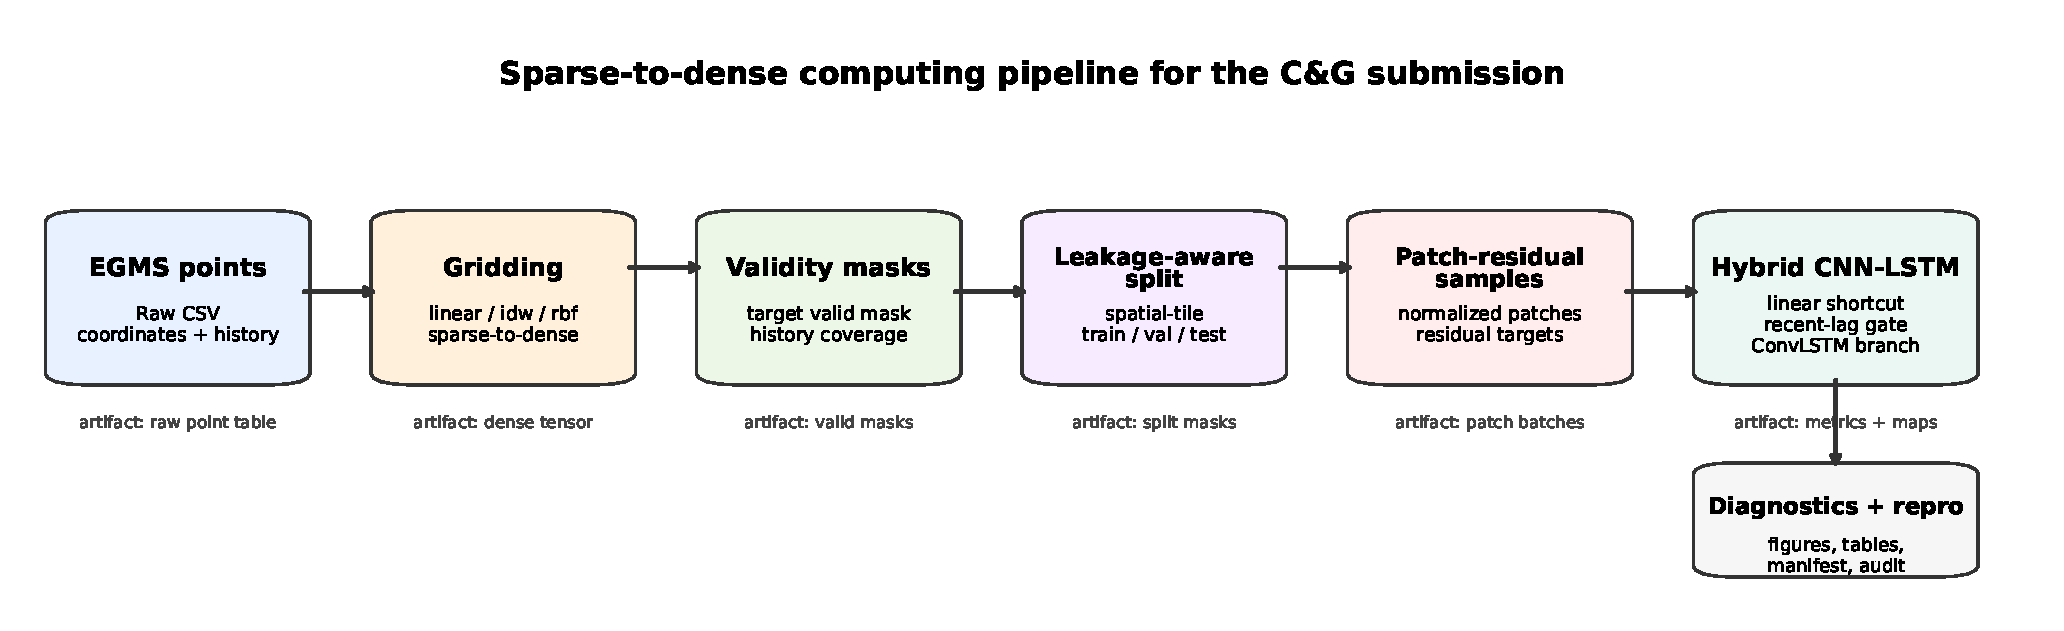
\includegraphics[width=\linewidth]{figures/fig01_pipeline_cageo.pdf}
\caption{Sparse-to-dense computing pipeline used for the C\&G submission. The figure highlights the full chain from EGMS points to gridding, validity masks, leakage-aware spatial-tile splits, patch-residual samples, the Hybrid CNN-LSTM backend, and the final diagnostics/reproducibility artifacts.}
\label{fig:f1}
\end{figure}

\begin{figure}[p]
\centering
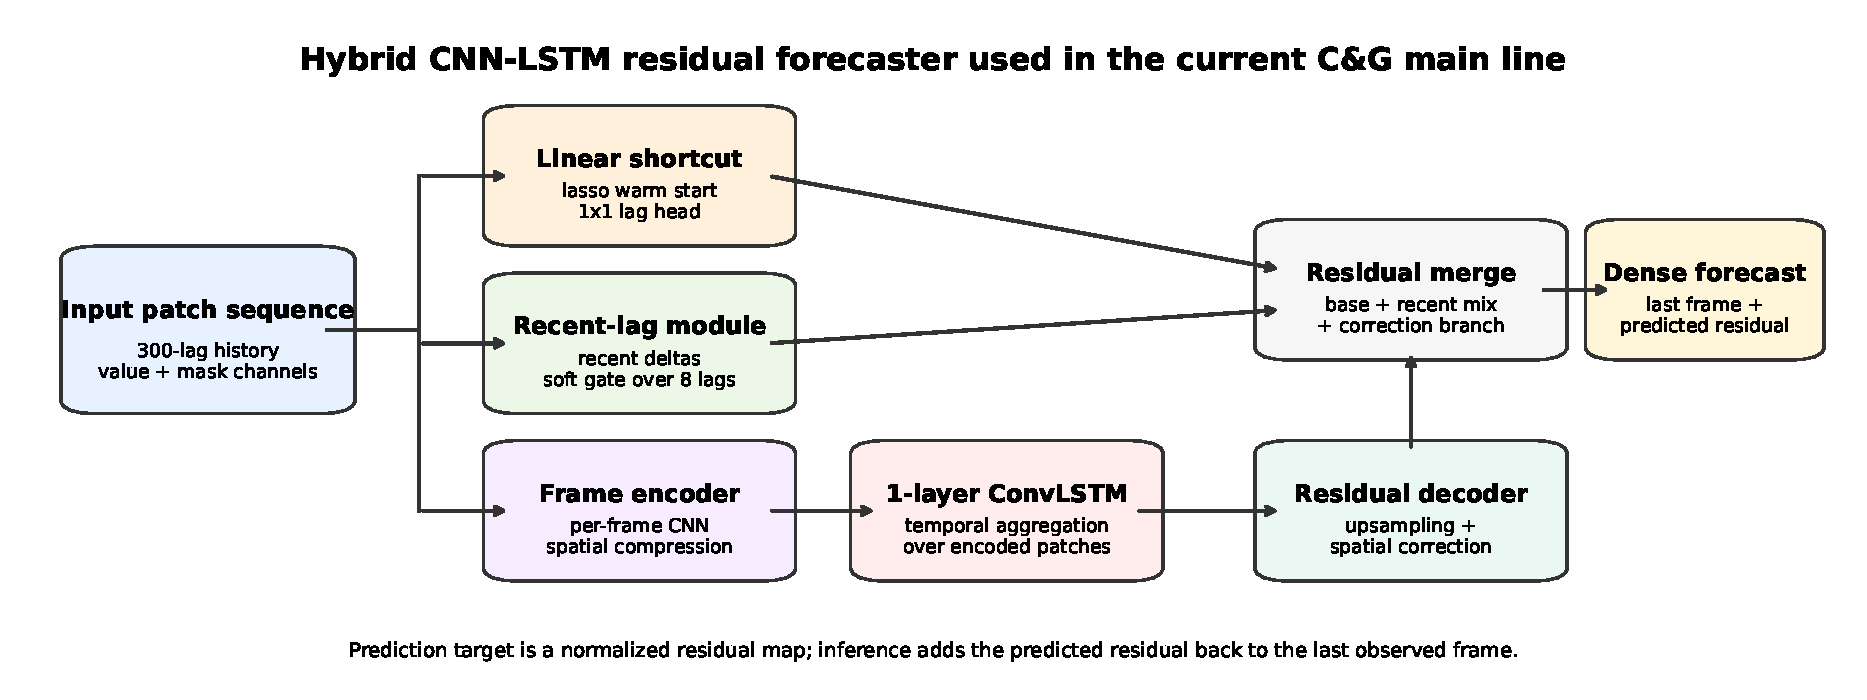
\includegraphics[width=\linewidth]{figures/fig02_hybrid_cnn_lstm_architecture.pdf}
\caption{Hybrid CNN-LSTM residual forecaster used in the current main line. The model combines a lasso-warm-started temporal shortcut, a recent-lag gating module, a one-layer ConvLSTM residual branch, and a spatial correction decoder. The final dense forecast is obtained by adding the predicted residual back to the last observed frame.}
\label{fig:f2}
\end{figure}

\begin{figure}[p]
\centering
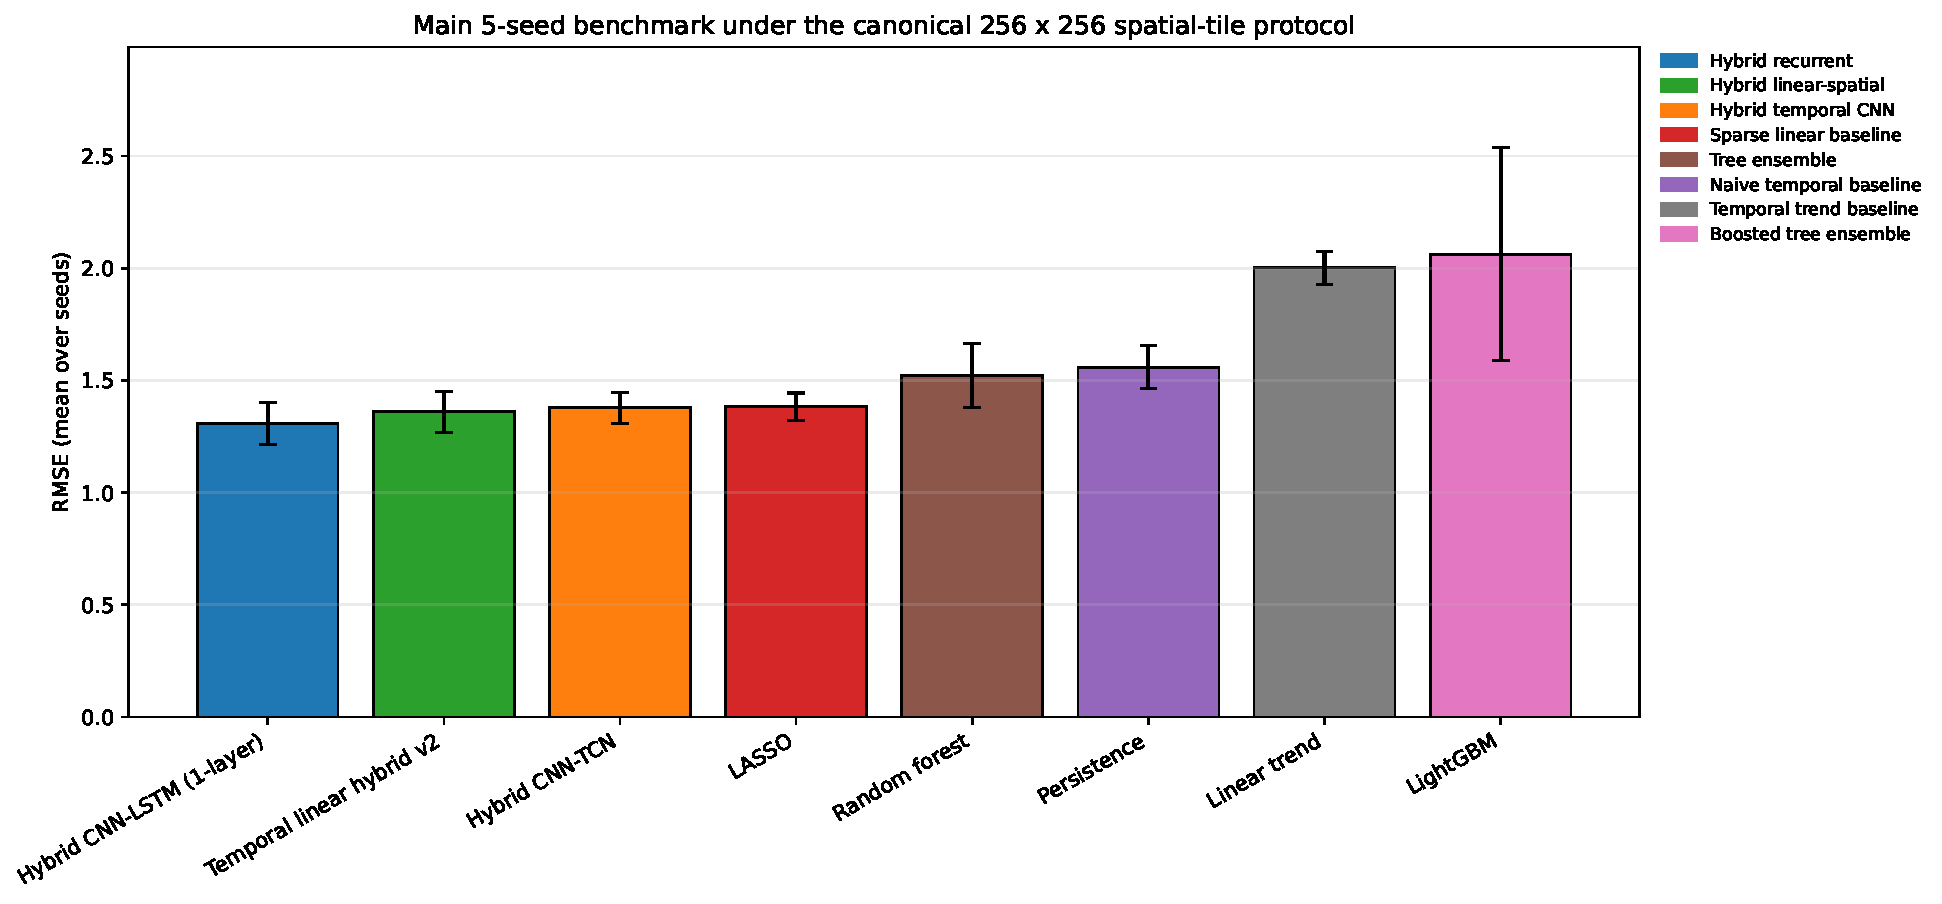
\includegraphics[width=\linewidth]{figures/fig03_main_benchmark_rmse.pdf}
\caption{Main benchmark RMSE with seed-to-seed uncertainty bars under the canonical 256 x 256 spatial-tile protocol with linear gridding. Bars are sorted by RMSE, and the proposed Hybrid CNN-LSTM (1-layer) is shown together with strong hybrid, linear, tree, and naive temporal baselines.}
\label{fig:f3}
\end{figure}

\begin{figure}[p]
\centering
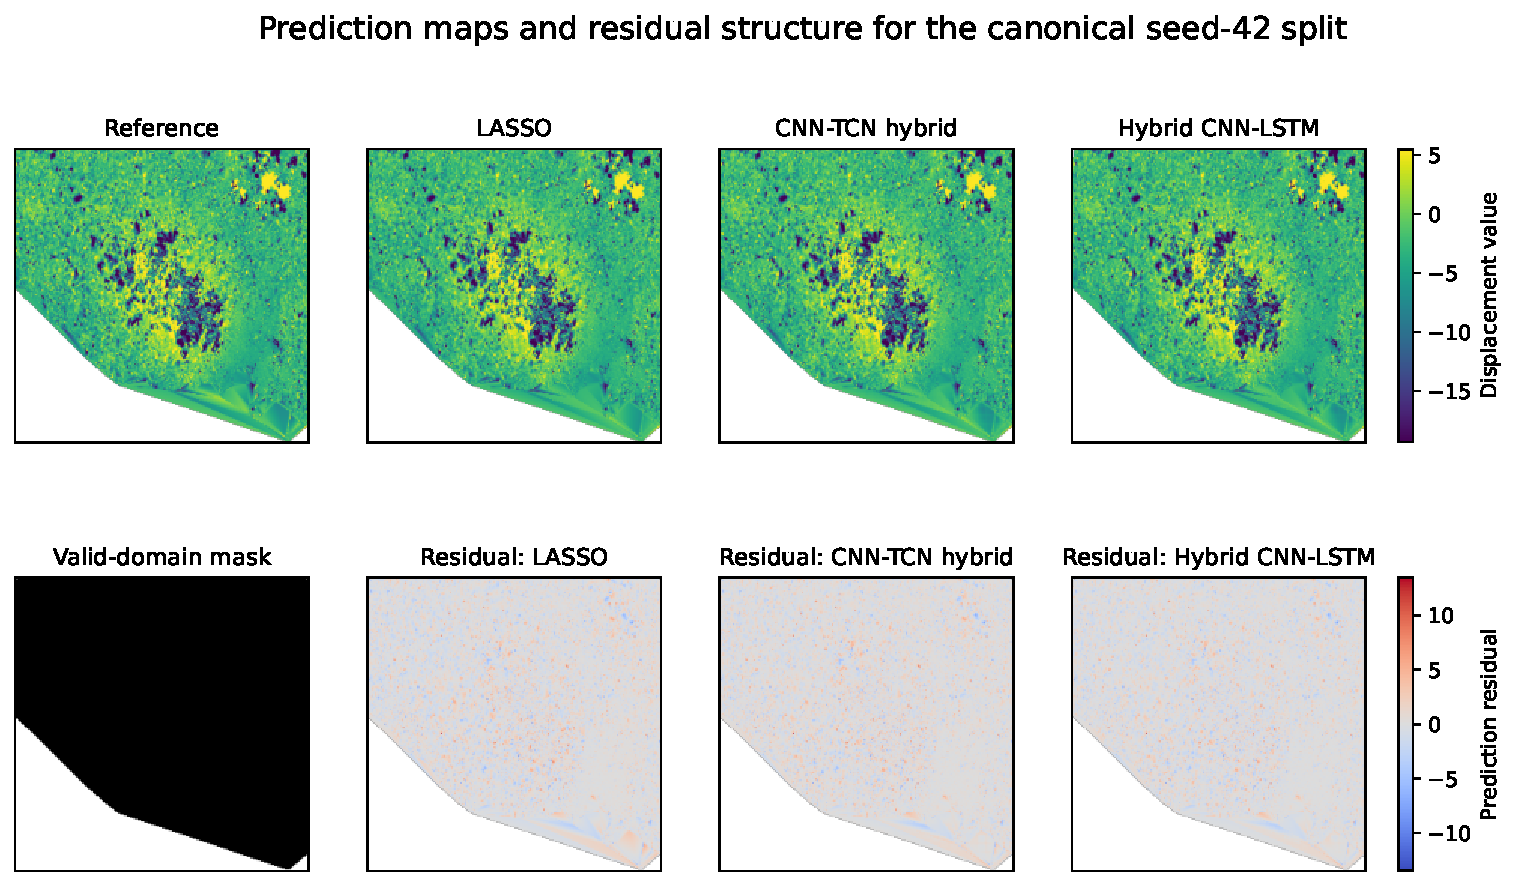
\includegraphics[width=\linewidth]{figures/fig04_prediction_residual_maps.pdf}
\caption{Prediction maps and residual maps for the canonical seed-42 split. The top row shows the reference map and the predictions of LASSO, the Hybrid CNN-TCN, and the Hybrid CNN-LSTM. The bottom row shows the valid-domain mask and model residual maps on a shared symmetric scale.}
\label{fig:f4}
\end{figure}

\begin{figure}[p]
\centering
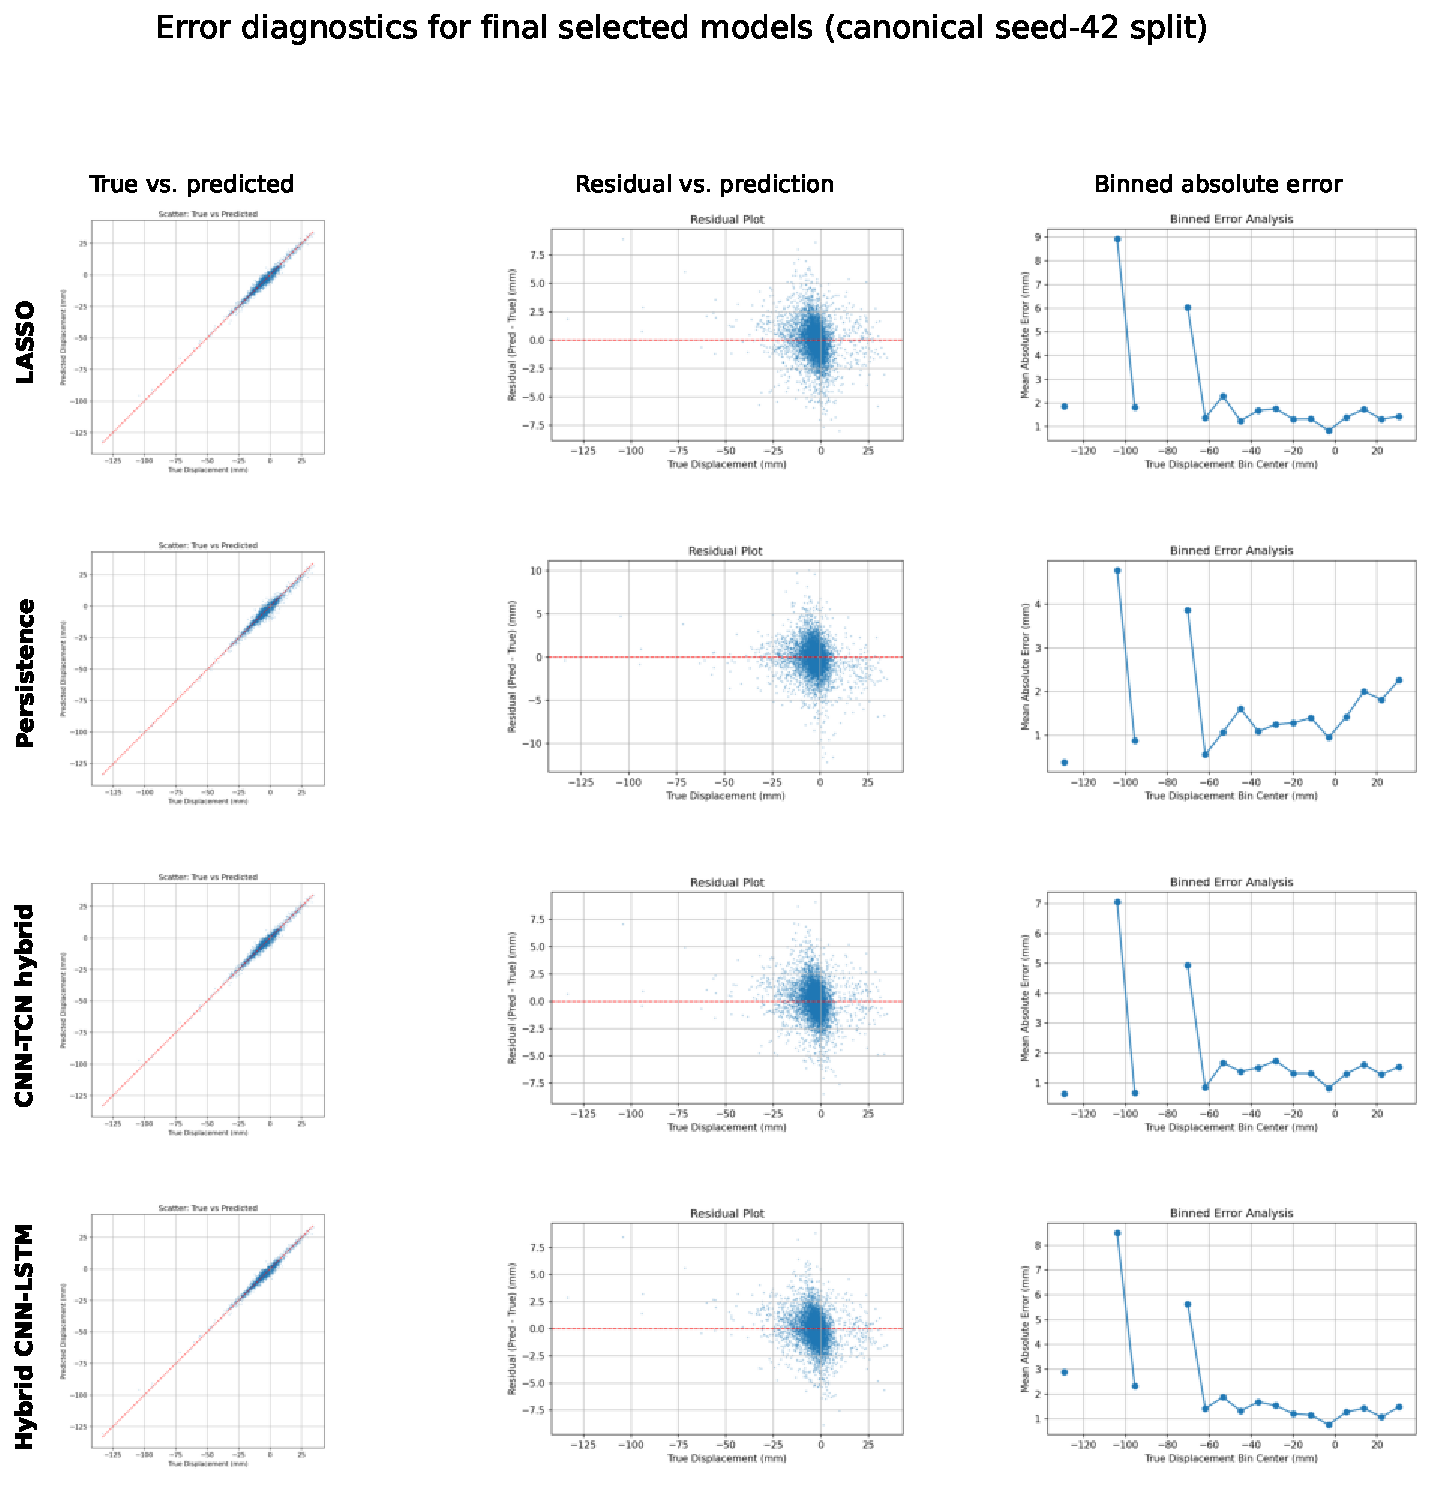
\includegraphics[width=\linewidth]{figures/fig05_error_diagnostics.pdf}
\caption{Error diagnostics for final selected models on the canonical seed-42 split. Each row corresponds to one model and each column shows the true-vs-predicted scatter, residual-versus-prediction plot, and binned absolute error summary.}
\label{fig:f5}
\end{figure}

\begin{figure}[p]
\centering
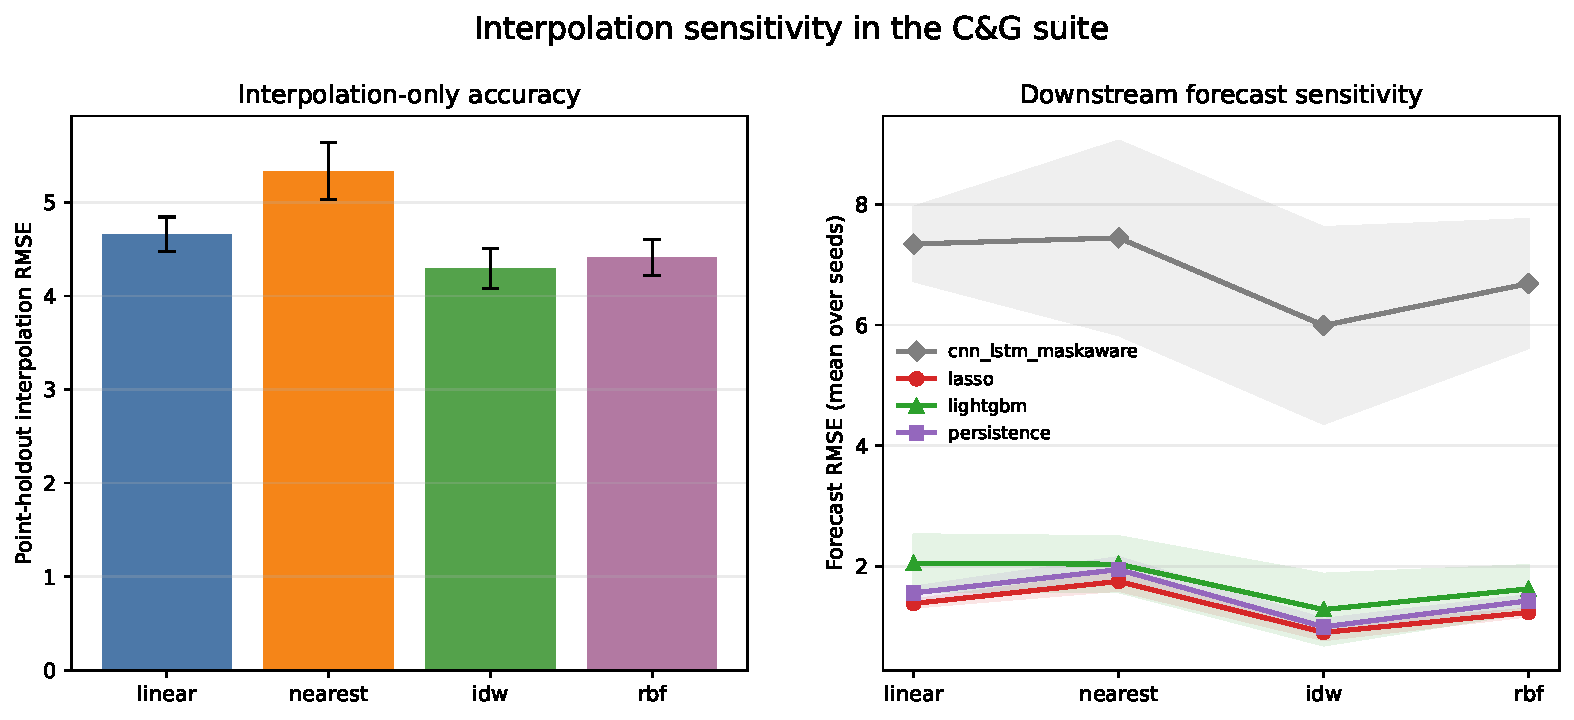
\includegraphics[width=\linewidth]{figures/fig06_interpolation_sensitivity.pdf}
\caption{Interpolation sensitivity in the C\&G suite. The left panel shows point-holdout gridding RMSE, and the right panel shows downstream forecast RMSE under aligned baselines. IDW is the strongest interpolation family in the current suite, but the final Hybrid CNN-LSTM has not yet been fully rerun under IDW for all five seeds.}
\label{fig:f6}
\end{figure}

\begin{figure}[p]
\centering
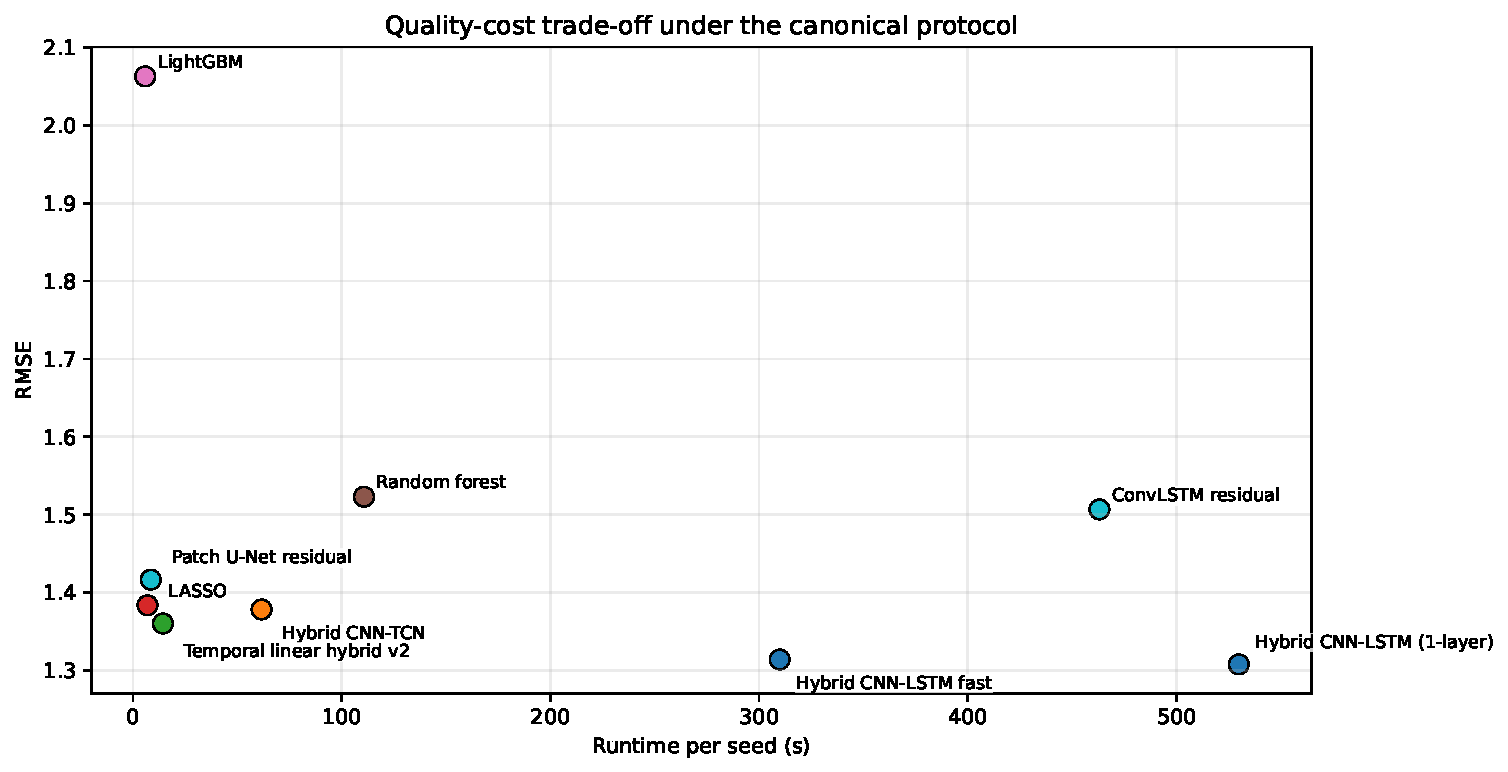
\includegraphics[width=\linewidth]{figures/fig07_runtime_rmse_tradeoff.pdf}
\caption{Runtime-RMSE trade-off across the main computational baselines and deep-learning routes. The figure highlights the quality-cost positions of the Hybrid CNN-LSTM main-quality configuration, its faster rerun configuration, the Hybrid CNN-TCN, and the strongest round-2 hybrid baselines.}
\label{fig:f7}
\end{figure}

\begin{figure}[p]
\centering
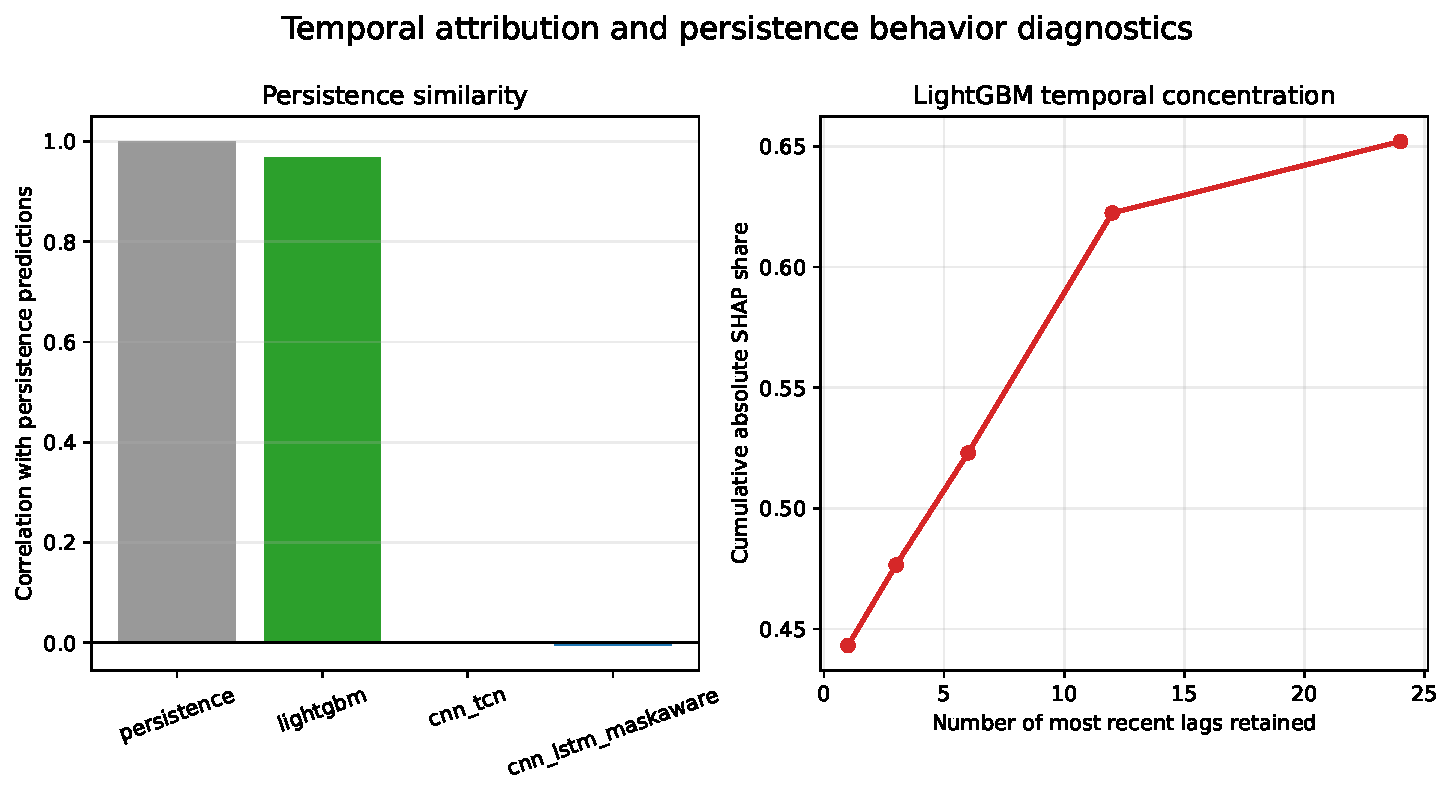
\includegraphics[width=\linewidth]{figures/fig08_persistence_similarity_or_shap.pdf}
\caption{Temporal attribution and persistence-behavior diagnostics. The left panel reports persistence-similarity correlations, and the right panel summarizes the cumulative share of absolute SHAP importance carried by the most recent LightGBM lags.}
\label{fig:f8}
\end{figure}

\begin{figure}[p]
\centering
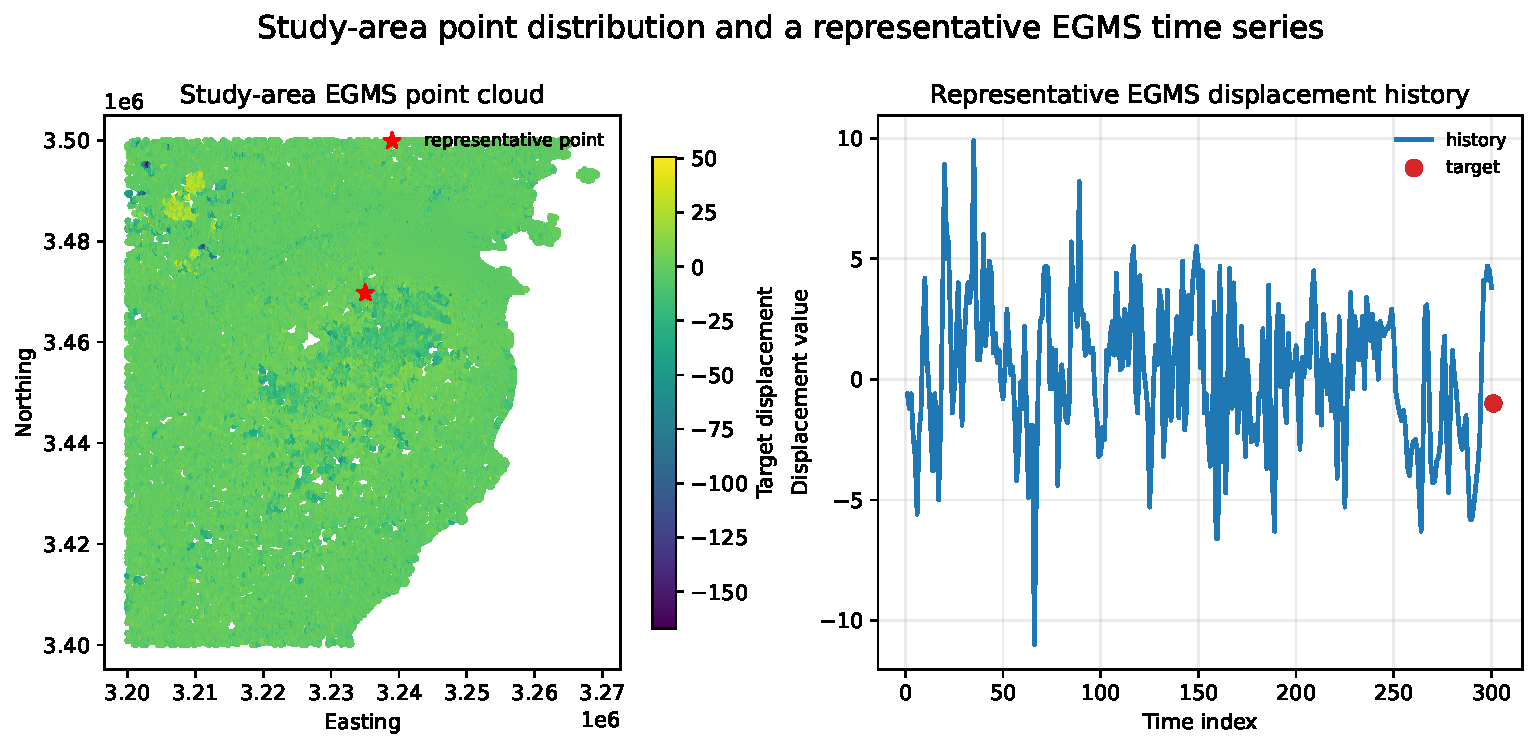
\includegraphics[width=\linewidth]{figures/fig09_study_area_timeseries.pdf}
\caption{Study-area EGMS point distribution and a representative displacement history. The left panel shows the sparse point cloud in projected coordinates, and the right panel shows a representative 300-step history together with its target displacement value.}
\label{fig:f9}
\end{figure}

\begin{figure}[p]
\centering
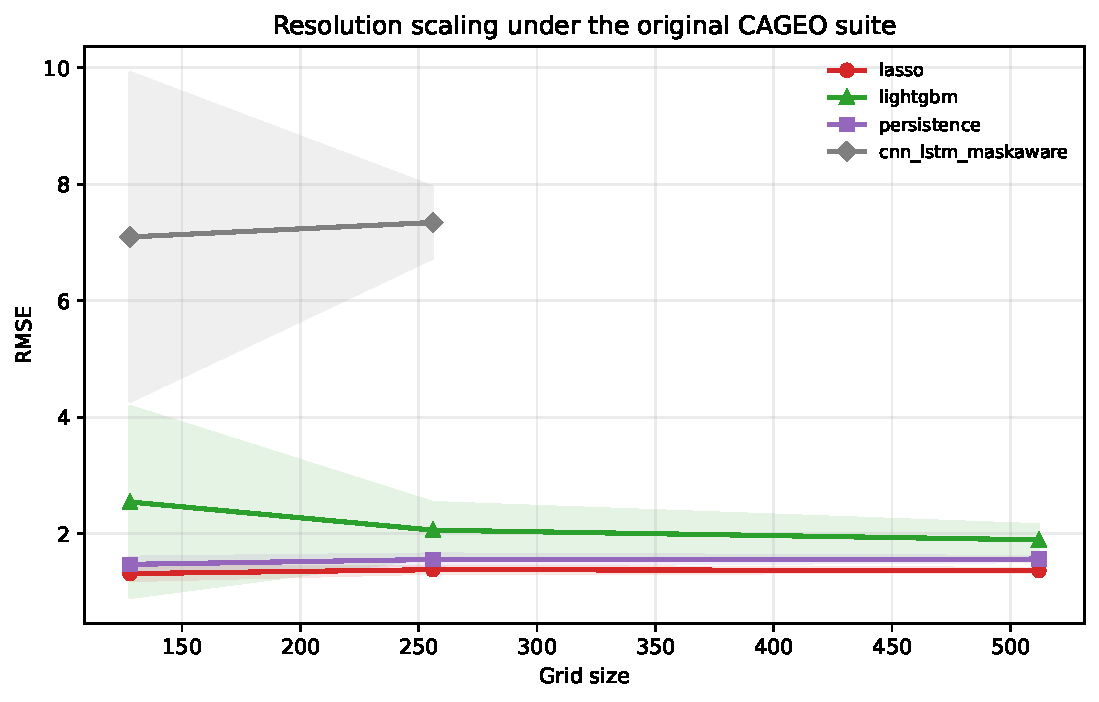
\includegraphics[width=\linewidth]{figures/figS01_resolution_scaling.pdf}
\caption{Resolution scaling from the original C\&G suite. The plot reports RMSE versus grid size for the strongest classical baselines and the obsolete early CNN-LSTM result where available.}
\label{fig:fs1}
\end{figure}

\begin{figure}[p]
\centering
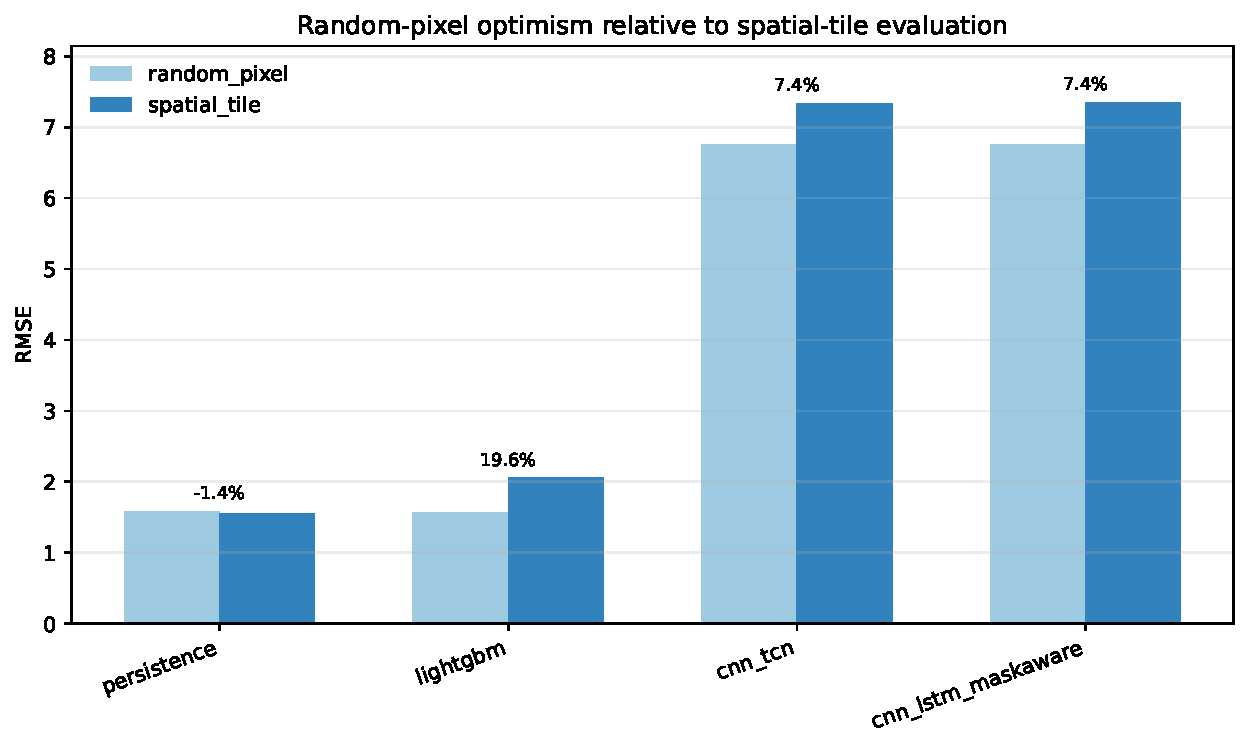
\includegraphics[width=\linewidth]{figures/figS02_split_leakage.pdf}
\caption{Split leakage comparison from the original C\&G suite. Random-pixel evaluation is systematically more optimistic than leakage-aware spatial-tile evaluation, particularly for LightGBM.}
\label{fig:fs2}
\end{figure}

\end{document}